\chapter{Getting Started}
\label{lab1}
\paragraph{} With the practical portion of this module we aim to learn about the functionality offered by the Android platform. We will treat each functionality as a building block which can be combined with other blocks, and glued together using the Java language to build our own apps. Throughout the practical labs we will explore these blocks and begin to combine them in simple ways. In your coursework assignment you will then have the opportunity to use these skills to design and implement an app of your own.

\begin{framed}
\paragraph{IMPORTANT} The libraries that make up the android platform are being continuously developed. Each new release is assocated with an API level. Higher API levels usually introduce changes that either break or deprecate working code from earlier level. The workbook currently targets API level 18 (codenamed Jelly Bean) which means that the code examples should be applicable to a cumulative distribution of around 70\% of real world devices. \emph{If you want to develop for a later API level, such as KitKat or Lollipop, in order to take advantage of more advanced features, particularly for your coursework assignment, then there may be instances of broken or deprecated code between the examples in the workbook and the android platform libraries.} However, for the core learning on this module we will assume that all of our development targets API level 18.
\end{framed}

\section{Aims}
\paragraph{} At the end of the practical portion of this topic you will be able to:

\begin{itemize}
\item Install the android development tools (OPTIONAL: Only if you have your own machine)
\item Create a default `Hello Android' application
\item Create an AVD for running your application
\end{itemize}

\paragraph{} We will use Android Studio to develop mobile applications on this module. Android Studio is an Integrated Development Environment (IDE) for managing the writing, testing, and running of Android applications. IDEs like Android Studio have many advantages when starting out with Android development. A lot of early activities when learning about Android is related to finding out what the platform offers. With an IDE there is usually a window or some code-completion that makes suggestions so that, over time, you become more familiar with the options available to you. There are particular advantages to using the command-line which are important, for example, when large teams of developers are working within a professional environment to collaboratively build applications. However, in this module we will concentrate on using an IDE.

\begin{framed}
\paragraph{IMPORTANT} \emph{This introductory practical is the only one which will describe in detail the process of creating a new project. All subsequent labs will assume that you can achieve this for yourselves. If in doubt refer back to this practical. It will be your responsibilty to explore and become familiar with your development environment so that you can at least perform basic tasks.}
\end{framed}

\begin{framed}
\paragraph{IMPORTANT} The code examples in the workbook are all included as source code in the module Git repository which can be found at: \url{https://github.com/siwells/teaching_set08114}. The workbook tries to focus on important aspects and fragments of a given topic but should not be used in isolation, rather, use the workbook to focus on fragments of the topic and the examples in the repository to see the fragment in the context of a full working app.
\end{framed}

\section{Say ``Hello Android''}
\label{hello}
\paragraph{} With an IDE there is a lot of initial hand-holding available to help get you started. In fact, to run a ``Hello World'' or more appropriately ``Hello Android'' app requires no code to be written at all. The entire app is generated ready to be compiled, installed, and run on an appropriate Android device such as connected hardware, emulator, or a virtual device. This is very useful because, depending upon the options that you select when you create a new app project, the basic scaffold for your app is automatically generated for you and is \emph{ready to run}, i.e. if you don't break it then Android Studio gives you a fresh, ready to run app (that does nothing very much). 

\paragraph{} This worksheet aims to give a pictorial introduction to the process of creating a first ``Hello Android'' application using Android Studio as your IDE. Studio actually does nearly all of the work for you and most of the time, at this stage in the module, all you need to do is {\bf{accept the defaults}}. So let's start by launching Android Studio.

\paragraph{} Use the `Quick Start' options in the right-hand pane and click `Start a new Android Studio project' as shown in Figure \ref{fig:android.studio_welcome}.

\begin{figure}[H]
\centering
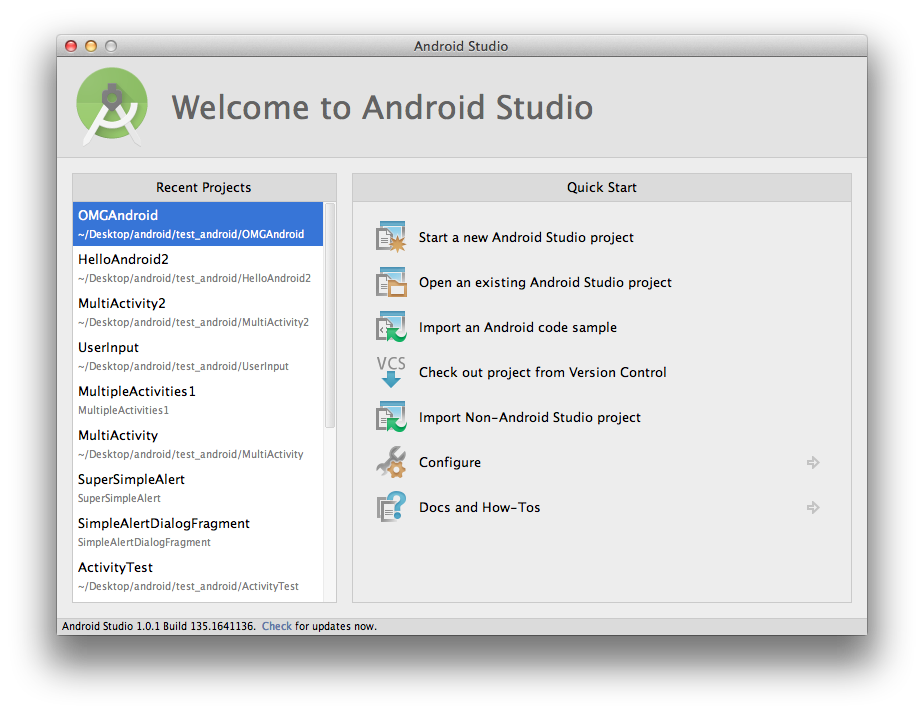
\includegraphics[width=\textwidth]{images/android-studio_01_welcome}
\caption{Android Studio welcome pane}
\label{fig:android.studio_welcome}
\end{figure}

\paragraph{} You should see the window shown in Figure \ref{fig:android.studio_config}. Enter a name for your new Application. This will also be used for your project name. For our first app let's call it `HelloNapier'. For `Company Domain' I suggest you enter `napier.ac.uk'. Now click Next to continue.

\begin{figure}[H]
\centering
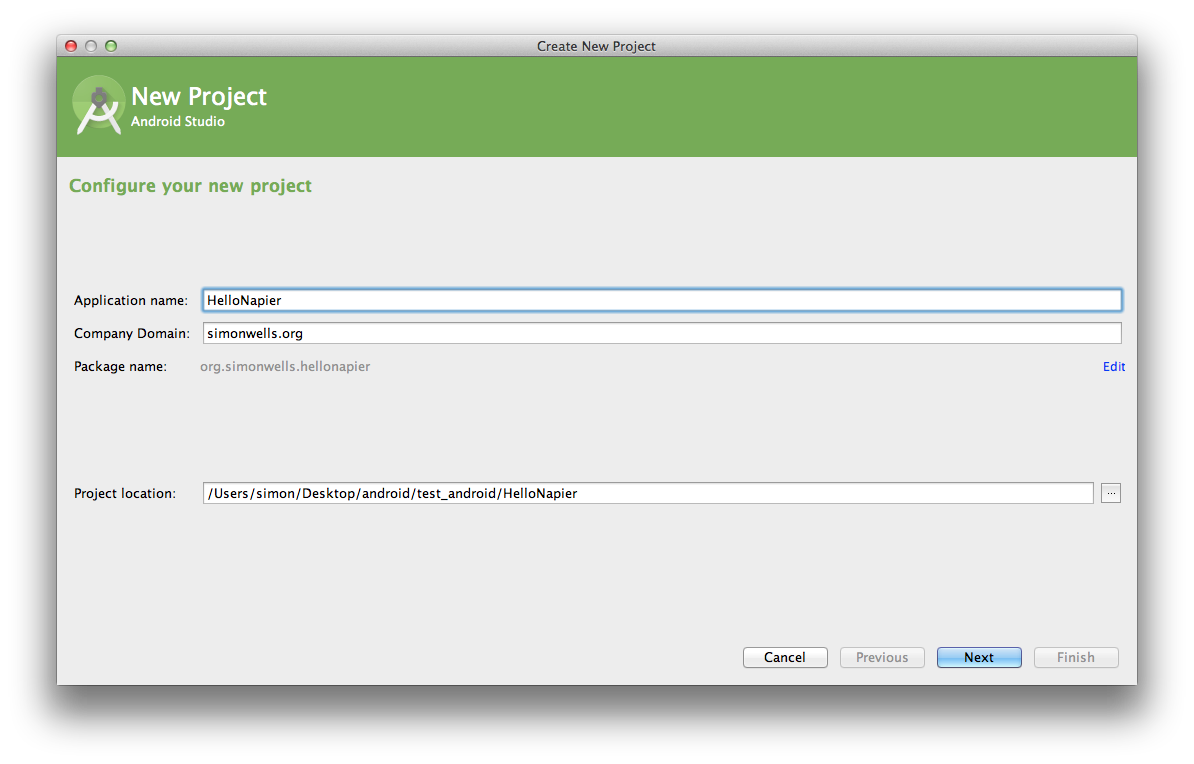
\includegraphics[width=\textwidth]{images/android-studio_02_configure}
\caption{Android Studio new app configuration pane}
\label{fig:android.studio_config}
\end{figure}

\paragraph{} On this screen, accept the defaults for now. NB. These should be as shown in Figure \ref{fig:android.studio_form}. Now click Next.

\begin{figure}[H]
\centering
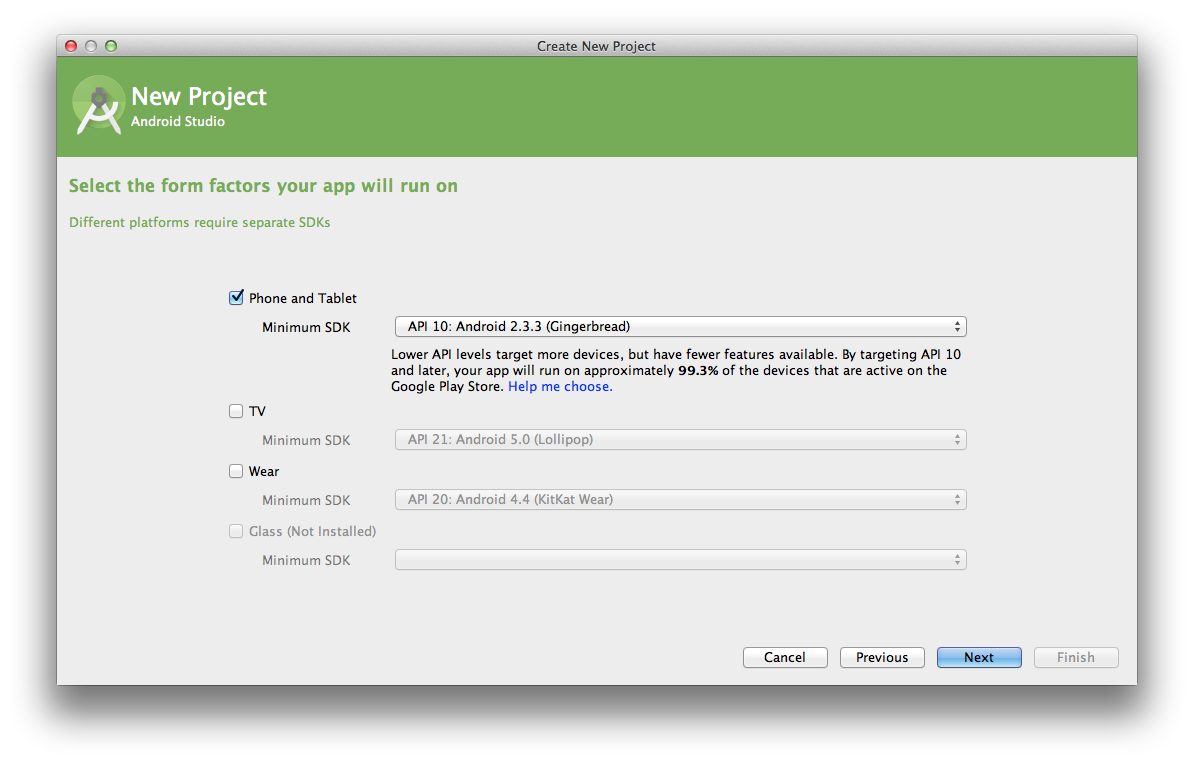
\includegraphics[width=\textwidth]{images/android-studio_03_form-factors}
\caption{Android Studio form factor selection pane}
\label{fig:android.studio_form}
\end{figure}

\paragraph{} Again, accept the default, `Blank Activity', which should be highlighted, then click Next.

\begin{figure}[H]
\centering
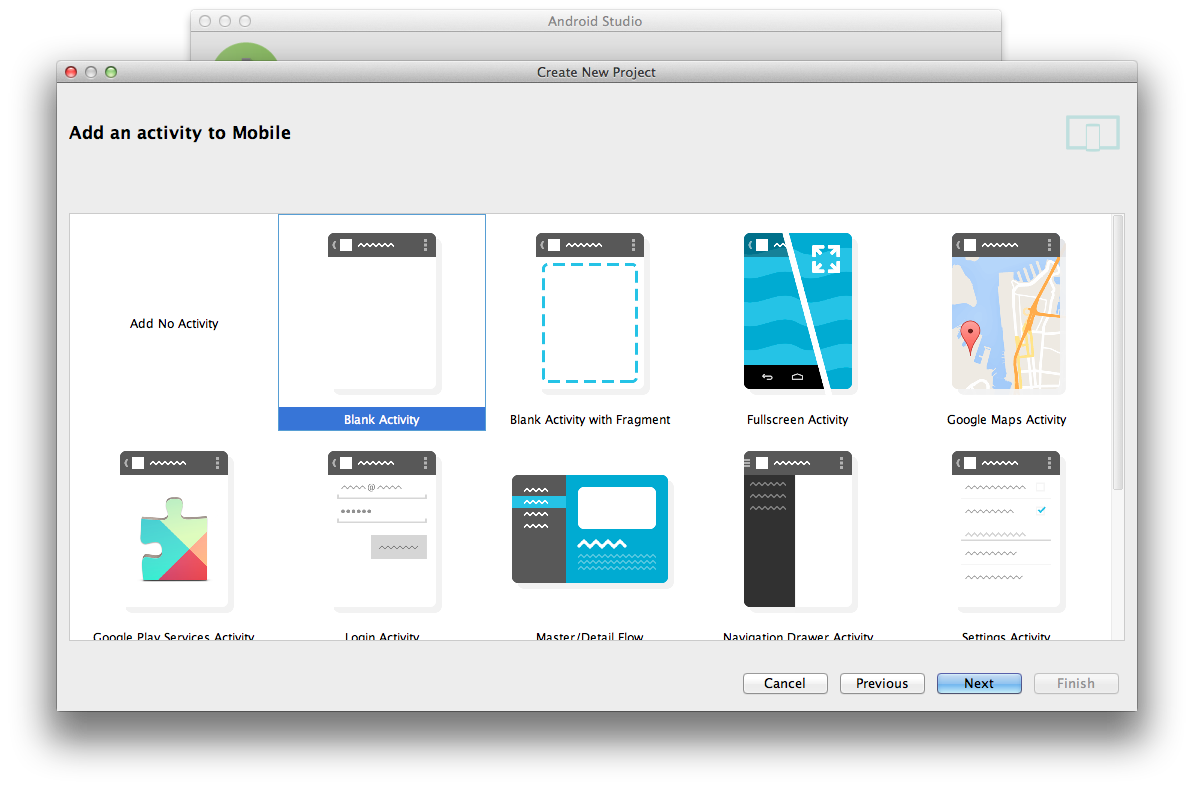
\includegraphics[width=\textwidth]{images/android-studio_06_activity}
\caption{Android Studio activity setting pane}
\label{fig:android.studio_activity}
\end{figure}

\paragraph{} Accept the defaults on this screen for now and click Next again.

\begin{figure}[H]
\centering
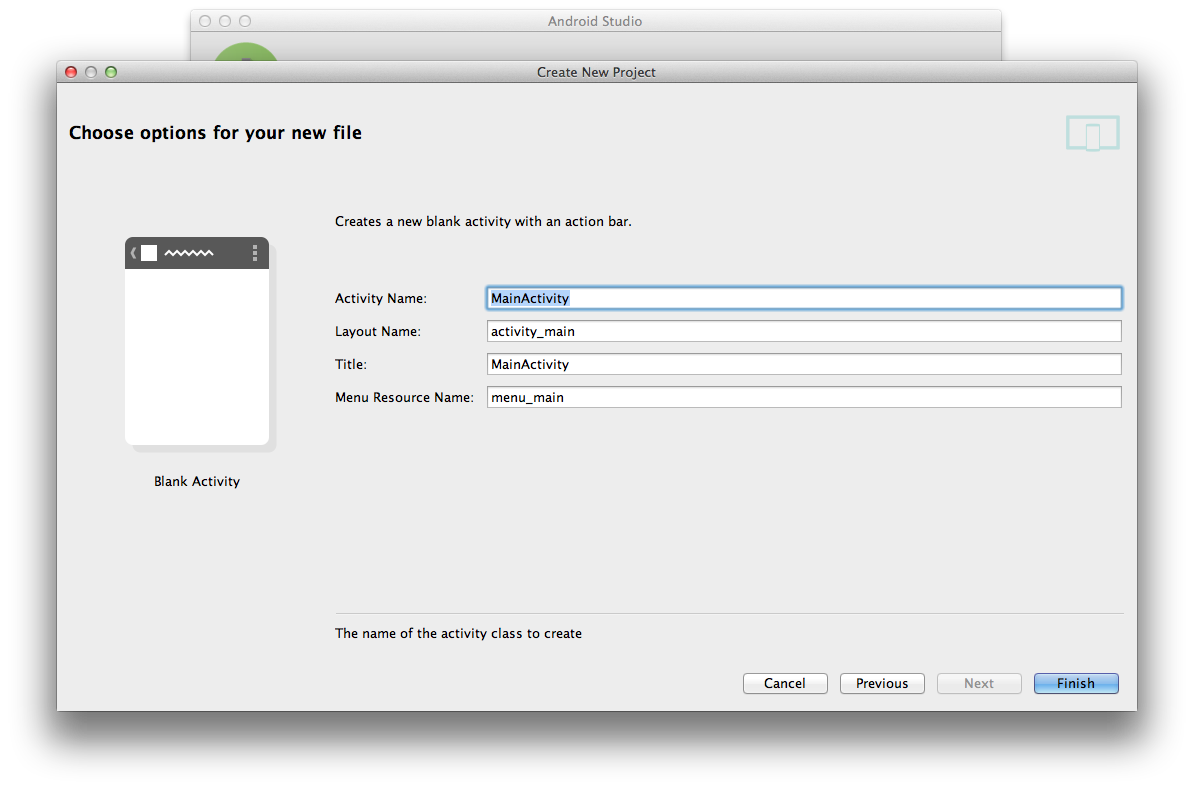
\includegraphics[width=\textwidth]{images/android-studio_07_options}
\caption{Android Studio options pane}
\label{fig:android.studio_options}
\end{figure}

\paragraph{} After a brief pause, whilst your machine loads all of the relevant libraries and creates your project file, you should be presented with the Android Studio workspace as shown in Figure \ref{fig:android.studio_studioui}.

\paragraph{NB.} It can take a while for your new project to load completely which depends upon the speed of your machine. If there are any errors or warnings on screen, especially in the preview window which renders waht your Android app interface will look like, then your project hasn't loaded completely yet.

\begin{figure}[H]
\centering
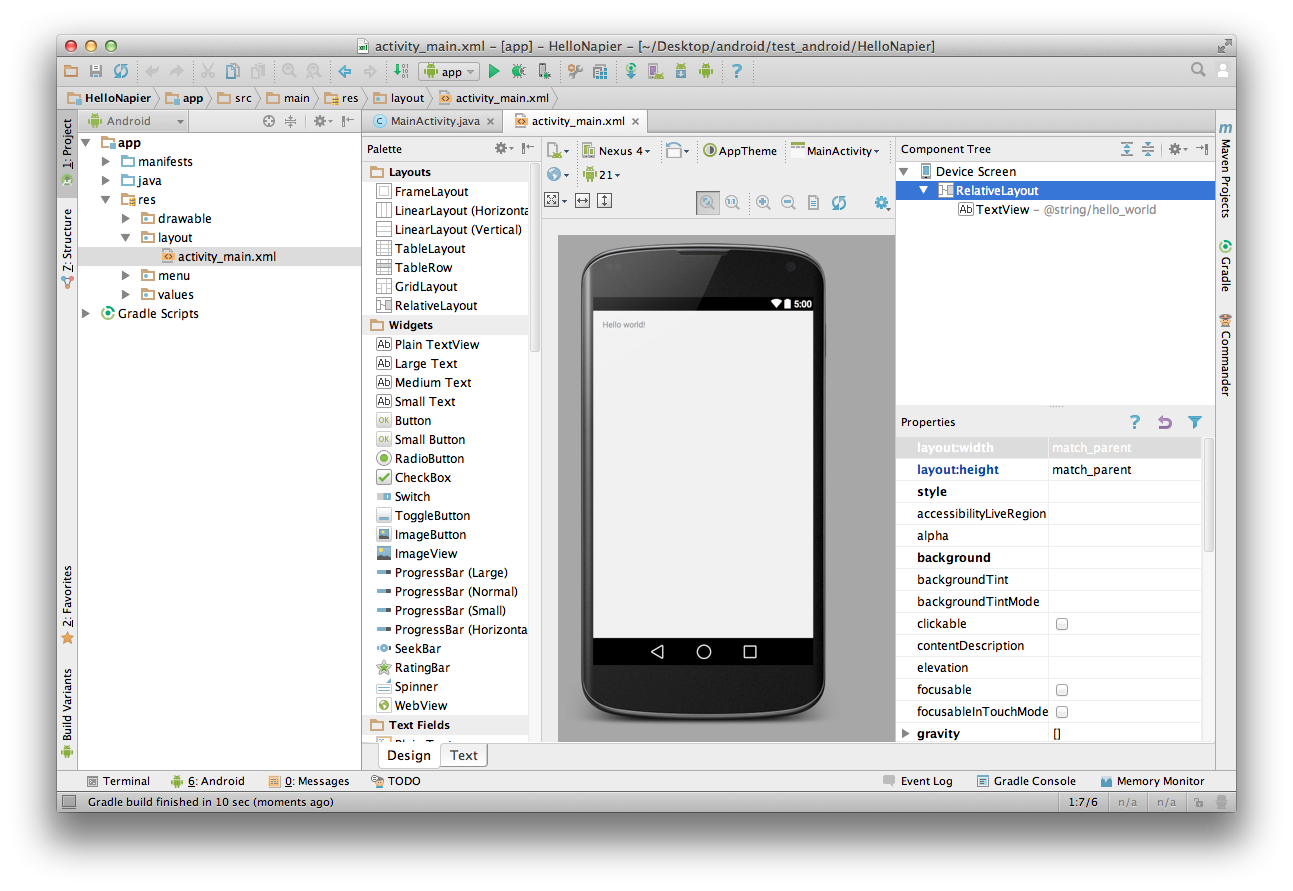
\includegraphics[width=\textwidth]{images/android-studio_08_studio-ui}
\caption{Android studio UI with default Android app}
\label{fig:android.studio_studioui}
\end{figure}

\paragraph{} Congratulations. You just created a New Android Studio projectThis process can be summarised as follows:

\begin{enumerate}
\item Click `Start a new Android Studio project'
\item Type in an application name \& Company Domain (napier.ac.uk) then click `Next'
\item Select an API level
\item Ensure `Blank Activity' is selected then click `Next'
\item Click Finish
\end{enumerate}

\paragraph{} Now you have created your first Android project. Whenever we say `Create a new project' we mean go though steps 1 to 5 ({\bf{you will have to either give each new project a different name or else save them to different locations}}).

\paragraph{} It is worth going through this process several times to become familiar with it. Once you have done it half a dozen times or so you should become comfortable with the idea of creating a new Android project and it shouldn't take more than a few seconds.

\paragraph{} It is also worth exploring some of the options that the project creation wizard offers. In particular it is worth exploring the API levels page to see what the differences are between the different API levels supported by Android. When you are on the form factors page shown in Figure \ref{fig:android.studio_form} click the link to ``Help me choose''. This will cause the API Level window to be displayed which is illustrated in Figure \ref{fig:android.studio_apilevel}.

\begin{figure}[H]
\centering
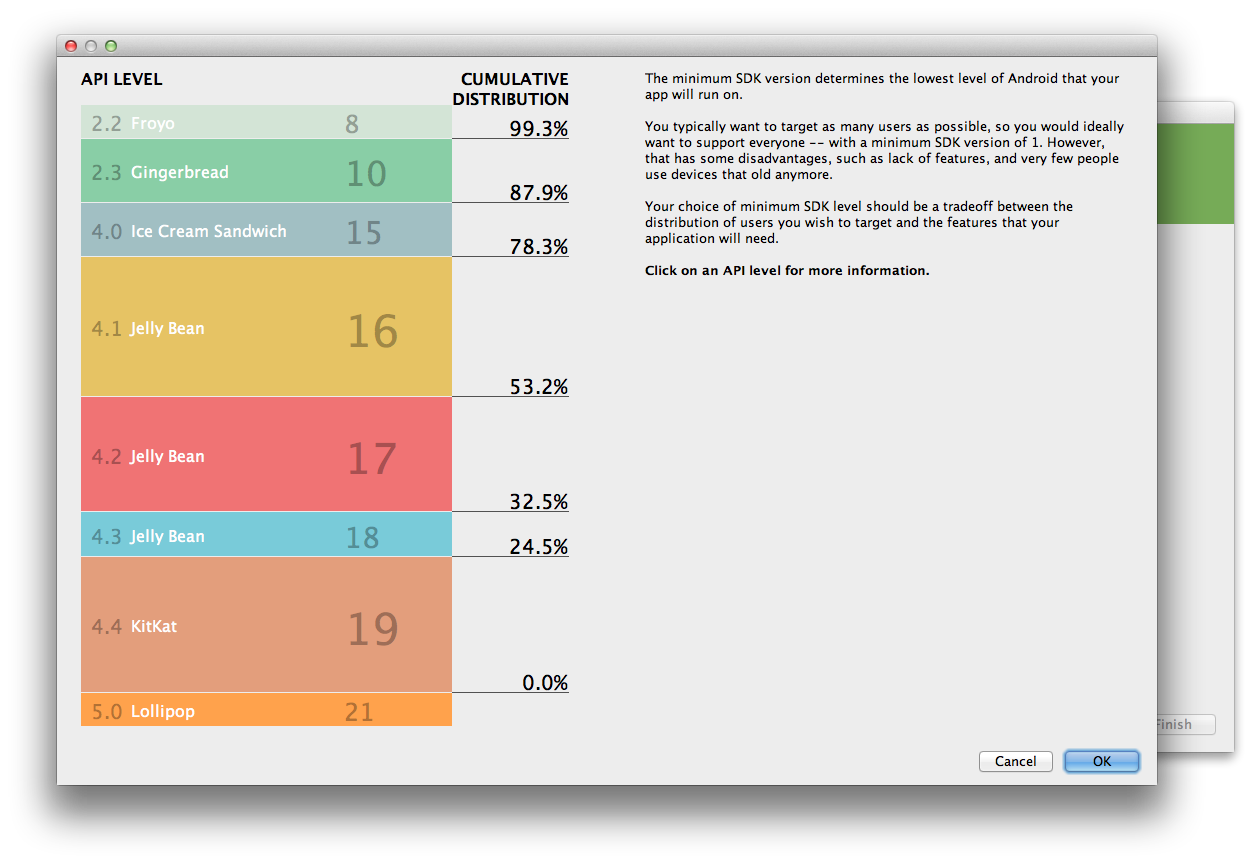
\includegraphics[width=\textwidth]{images/android-studio_04_api-level}
\caption{Android Studio API level selection screen}
\label{fig:android.studio_apilevel}
\end{figure}


\paragraph{} This page gives you an idea of the proportion of the market for Android devices that you can target with each API level. If you click on a particular level, e.g. `2.3 Gingerbread' then you will see extra information about the features offered by that verson of Android. Remember, higher API levels support newer or more refined features whereas lower levels are supported by a wider proportion of the population of Android devices. Choosing an API level is therefore partly a technical decision, because it affects what you can do, partly a business decision, because it affects the size of your potential customer base, and partly an aesthetic decision, because how things are displayed is also affected by API level. So choose wisely ;) 

\begin{figure}[H]
\centering
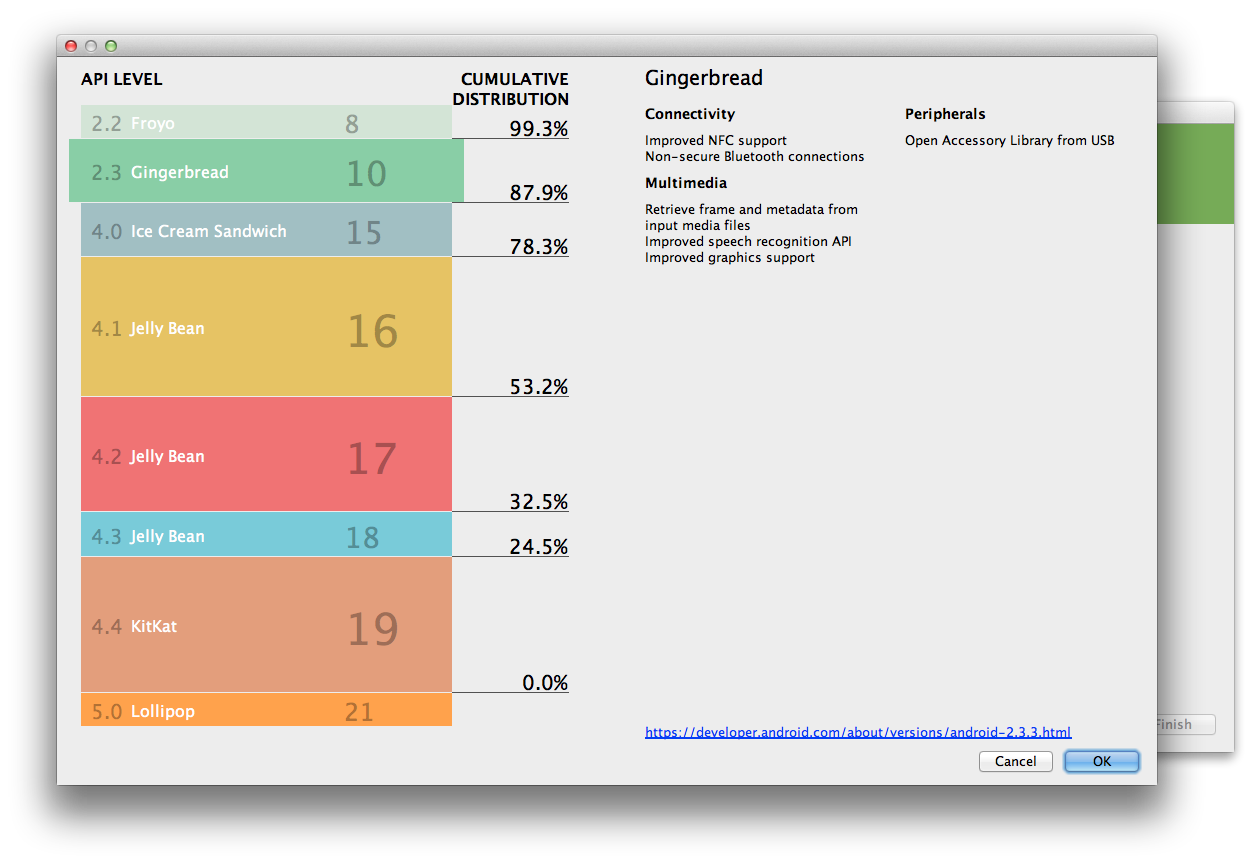
\includegraphics[width=\textwidth]{images/android-studio_05_api-level-details}
\caption{Android Studio API level details screen}
\label{fig:android.studio_apidetails}
\end{figure}

\paragraph{} It can take quite a while, even minutes, for Android Studio to completely load your new project and all of the supporting libraries. If the preview of the Android UI isn't fully displayed or has a message on it then Android Studio is still loading and compiling things so it is best to let it finish. Similarly if there are errors or warnings in the ``Problems'' tab then it is likely that these are due to your IDE still loading and building resources. Sometime the IDE can also get ahead of itself and tries to use one component before another is properly loaded. Usually when this occurs there will be a message with a link to let you reload or retry the component. When we build a new Android Studio project, especially for the first time, there will be a lot of code to generate and libraries to link, and this can take a while. Also, because everyone in the class is trying to do this at the same time, and Android Studio runs across the university network from the ``U:\'' drive there can be some significant lag. At this point you should just wait for things to resolve themselves. You imght also notice, in the status bar of Android Studio, that there is a message regarding scanning or indexing files, this happens when we first use Android Studio, it can take a while to complete, and it can cause significant performance issues initially.

\paragraph{} Now you need to build and run your app. This is important because we want to actually see our app running and doing something don't we?

\section{Running our app using Android Virtual Devices (AVDs)}
\label{avd}
\paragraph{} Because Android apps are not Windows (or Linux, or MacOS) apps they will not usually run natively on our operation systems (unless you are using Android as your OS but let's ignore that case for now). That means that you cannot just double click on your app and have it run in a window. Android apps rely on the Android OS to provide not just the platform libraries that contain all the code you didn't write but also all of the app management functionality. Android apps are a collection of activities (we will talk about these in class next week) and the OS manages when to display a given activity and when to allow another activity to take precedence. As a result we need a way to run our Android app. There are three alternatives, you can use a hardware device plugged into your computer via USB, or you can emulate the hardware of an Android device. Android devices usually run on an ARM architecure, which is different to most desktop machines, and thus that architecture needs to be emulatedin software, this can be very slow. A third option is to use a virtual device that runs a version of the Android OS that is built for the x86 architecture. This allows us to use real hardware, e.g. CPU cores and RAM, to run the Android OS in the virtual device. We can then load our Android app in this virtual version of Android and have it run with acceptable performance. This approach is known as using an `Android Virtual Device' (AVD) and we interact with AVDs through the AVD manager. We can access this through the Tools $\to$ Android $\to$ AVD Manager menu option. The AVD manager lets you set up multiple AVDs, e.g. targetting different versions of Android or simulating different hardware capabilities. For the moment we should merely use the default AVD and accept the defaults that the AVD manager suggests. Bare in mind that an AVD is quite large, around 650MB each, so you might not want to create too many of them. Currently AVDs are stored in the C: drive of the JKCC machines so each time you use a different machine you will probably have to create a new AVD. This is a known ``feature'' of the JKCC which is being worked on. 

\paragraph{} Once you have created a new Android device then it it needs to be started. As this process is essentially starting up a whole operating systems this can take a few moment. Eventually however you should see a new window that looks a bit like an Android device

\paragraph{} Once you have an AVD created you can select the Run $\to$ Run `app' menu optionand your Android app will be built and tranferred to your AVD. You might have to select the AVD that you want to run the app in from a list of running devices. NB. If you have attached a harware device to your computer using USB then this device should also be listed however there are some caveats; you will need to have the correct drivers installed for your device and this will probably not work in the JKCC with your own device but should be OK on your own laptop.

\paragraph{} That's it for this week. You should get yourself \emph{very} comfortable with these processes and go through them multiple times as every app that you will build during the mdule, and you will build tens if not hundreds of apps, will require you to set up a new project. You should only need a single AVD using the default settings for the majority of the lab exercises. If other settings are required for a particular exercise then this will be flagged as necessary. That said, experiment with Android studio, explore some of the features that it offers, and get as familar as you can with it so that you are ready to do more in subsequent labs.


